\chapter{Programmable realtime unit}
\label{chap:pru}

This chapter will discuss the capabilities, and usage of the Programmable Realtime Unit (\textls{PRU}).

Even with realtime operating systems, no process can take up hundred percent time of a CPU. There are essential OS management tasks, which handles the hardware. These management tasks need to be executed periodically.

\section{Example}
\label{subsec:example}

This example illustrates the usability of an external control unit, if the system has rigorous timing criteria.

\begin{figure}[h]
	\centering
	\begin{tikzpicture}[
			label/.style={
				font=\footnotesize
			}
		]
		\node[squarednode] (A) [] {\rtos};
		\node[squarednode] (B) [right = 4cm of A] {Controller};

		\draw[thick,->] (A.east) -- ++(4,0) node[above,pos=0.12] (AB) {};
		\draw[very thick,->] (B.east) -- ++(4,0) node[midway,above,text width = 3cm] {To controlled unit};
		\timing at (AB) {6{1C 0.5C}C};
	\end{tikzpicture}
	\caption{A bit--banging solution for PWM}
	\label{fig:example_pwm}
\end{figure}

\cref{fig:example_pwm} depicts the example. Our example consist of a computer (\rtos), and a controller. The \rtos component is sending a pulse width modulated signal (\pwm) to the controller. The controlling computer does not have an integrated \pwm controller, and the signal modulation must done by software. This method when a typically hardware implemented peripheral is emulated called \emph{bit--banging}.

In use cases where the controller needs a very precise signal, because a small change in the width of the modulated signal cause a big difference in the output of the controller. This means the solution needs the smallest reachable jitter.

This example relies on the measurements of \citep{rt-sched-thesis}, which uses the same development platform this chapter will discuss. It is important to point out the measurements were done on a soft real--time OS. Other commercial products which specializes in hard real--time (VxWorks, µC/OS-II) might reach better performance, but this chapter will reveal alternate solutions.

\subsection{Evaluation}

At PWM period of 50ms, the system was capable generating accurate control signal from software. At 10ms, the best achievable jitter was $1.32\%$, and at 1ms, $4.1\%$.
Because the computer is not totally dedicated to generate our control signal, jitter can happen. If the specified system requires low jitter, this solution may not be applicable to the design.

\section{Delegation of real--time functionality}

One possibile solution for \cref{subsec:example} is to delegate this task to an external coprocessor.

\begin{figure}[h]
	\centering
	\begin{tikzpicture}
		\node[squarednode] (A) [text width=1.5cm] {\rtos};
		\node[squarednode] (B) [below = 1.5cm of A] {Microcontroller};
		\node[squarednode] (C) [right = 2cm of B] {Controller};

		\draw[thick,->] (A) -- (B) node[midway, right] {Commands};
		\draw[thick,->] (B) -- (C) node[above,pos=0.12] (AB) {};
		\draw[very thick,->] (C.east) -- ++(3.7,0) node[midway,above] {To controlled unit};
		\timing[timing/slope=.25] at (AB) {3{0.8C0.4C}C};
	\end{tikzpicture}
	\caption{An external microcontroller as PWM signal source}
	\label{fig:example_external_pwm}
\end{figure}

With this approach the design have an external component. This component, usually a microcontroller, is a completely separate unit. The communication between these units can be done with protocols designed to tolerate errors in timing e.g. the Inter-Integrated Circuit (\isc) protocol.

The only job of the microcontroller is to generate the corresponding controlling signal. This is a far more controlled environment, because microcontrollers don't usually run operating systems\,--and while interrupt handling might cause problems\,--the order of robustness is definitely higher than RTOS based solutions.

On the downside, the design have an additional external component which is an overhead in the design and programming process. The optimal solution would be to merge the two processors into one.

\section{Programmable realtime unit}

Instead of having an external controller (\cref{fig:ext_controller_hw}), this external coprocessor could be integrated into the integrated circuit of the central processing unit (\cref{fig:int_controller_hw}).

This can be beneficial because we need less external components, and because of the integrated property of this solution, the communication with the coprocessor is reliable.

Additionally the coprocessor can use some of the resources of the host \cpu which would be hardly accessed in an external configuration.

\begin{figure}[h]
	\centering
	\begin{tikzpicture}
		\node[squarednode] (A) [] {Main computing unit};
		\node[squarednode] (B) [right = 4cm of A] {External controller};

		\draw[thick,<->] (A.east) -- ++(4,0) node[midway,above] (AB) {Commands \& Data};
	\end{tikzpicture}
	\caption{External coprocessor}
	\label{fig:ext_controller_hw}
\end{figure}

\begin{figure}[h]
	\centering
	\begin{tikzpicture}[
			innernode/.style={
				minimum height=1cm,
				text width=2.8cm,
				align=center
			}
		]

		\node[squarednode, innernode] (ECU) [] {Embedded controller};
		\node[squarednode, innernode] (MCU) [left = of ECU.west] {Central processing unit};
		\node[squarednode] (A) [ultra thick, fit=(ECU) (MCU), inner ysep=5mm, inner xsep=5mm] {};

		\node [above = 2mm of A.south] {\textbf{\large IC}};

		\draw [thick,<->] (ECU.west) -- (MCU.east);
		\draw [thick,<->] (MCU.north) -- ++(0, 1);
		\draw [thick,<->] (ECU.north) -- ++(0, 1) ;
	\end{tikzpicture}
	\caption{Integrated coprocessor}
	\label{fig:int_controller_hw}
\end{figure}

\subsection{AM335x processor family}

The AM335x is the Texas Intruments' ARM Cortex-A8 processor family \citep{AM335x}. This thesis will focus on the AM3358 processor, because the BeagleBone Black \citep{BBB} has this \cpu. The BeagleBone Black is the reference system this case study will use.

The AM335x processor family have four member (AM3359, AM3358, AM3357, AM3356) which have special unit called \emph{Programmable Realtime Unit and Industrial Communication SubSystem} (\pruss). A \pruss consists two \emph{Programmable Realtime Unit} (\pru). These units are Hardware architecture based microcontrollers which can be programmed by an application running on the central processing unit.

The \pru is not an accelerator next to the media processor, it's sole purpose is to offload hard real--time software components into these units. In this way, the designer may avoid the usage of a real--time operating system, which can be a big tradeoff in performance, capabilities, design and license costs.

\needspace{10\baselineskip}
The basic properties of the AM335x \pruss (be warned, there are previous generations of \pruss, generations do not always indicated):
\begin{itemize}
	\item 2 \pru processor per \pruss:
	\begin{itemize}
		\item \SI{32}{\bit} Harward architecture, without pipelining
		\item \SI{200}{\mega\hertz} clock speed, all instruction executed in \SI{5}{\nano\second}
		\item \SI{8}{\kilo\byte} instruction memory
		\item \SI{8}{\kilo\byte} data memory
		\item \SI{12}{\kilo\byte} shared memory between the two processor
		\item Up to 17 input, and 16 output
	\end{itemize}
	\item An interrupt controller shared between the \pru cores
	\item Access to the system peripherals, e.g.: DRAM, GPIO
	\begin{itemize}
		\item System DRAM access is possible, but nondeterministic
		\item GPIO handling is direct, meaning I/O can be handler with \SI{5}{\nano\second} resolution.\footnote{The sustainable maximal frequency achievable is \SI{50}{\mega\hertz}, because the toggle loop takes 4 instructions to execute.}
	\end{itemize}
\end{itemize}

\begin{figure}[h]
	\centering
	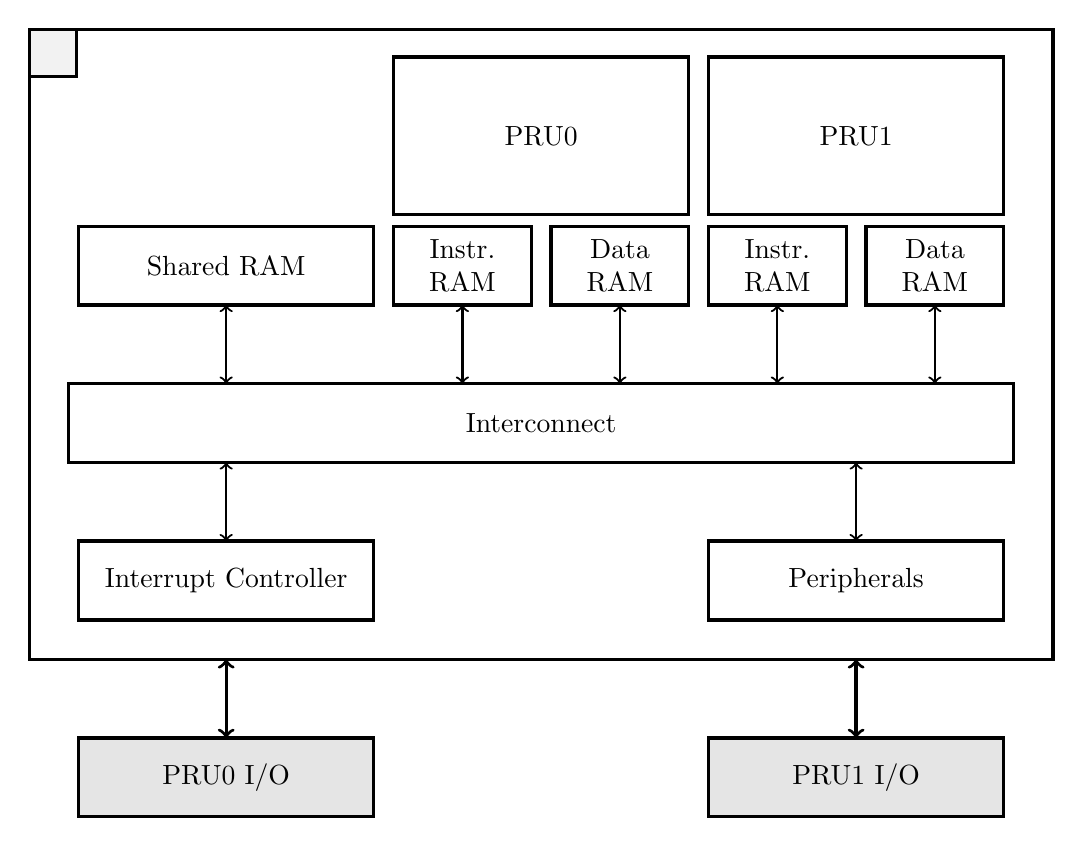
\begin{tikzpicture}[
			squarednode/.style={
				rectangle,
				draw=black,
				very thick,
				align=center,
				inner sep=0cm
			},
			main/.style={
				minimum width=13cm,
				minimum height=8cm
			},
			interconnect/.style={
				minimum width=12cm,
				text width=12cm,
				minimum height=1cm
			},
			sram/.style={
				minimum width=3.75cm,
				text width=3.75cm,
				minimum height=1cm
			},
			ram/.style={
				minimum width=1.75cm,
				text width=1.5cm,
				minimum height=1cm
			},
			pru/.style={
				minimum width=3.75cm,
				text width=3.5cm,
				minimum height=2cm
			}
		]

		\node[squarednode,main] (Box) at (0,1) {};
		\node[squarednode,below right,inner sep=3mm, fill = black!5] at (Box.north west) {\large\textbf{\pruss}};

		\node[squarednode,interconnect] (SharedRam) at (0,0) [] {Interconnect};

		\node[squarednode,sram] (IntC)  at (-4,-2) {Interrupt Controller};
		\node[squarednode,sram] (Peri)  at (4, -2) {Peripherals};

		\draw[thick, <->] (-4,-1.5) -- (-4,-0.5);
		\draw[thick, <->] (4, -1.5) -- (4, -0.5);

		\node[squarednode,sram, fill=black!10] (IntC)  at (-4,-4.5) {PRU0 I/O};
		\node[squarednode,sram, fill=black!10] (Peri)  at ( 4,-4.5) {PRU1 I/O};

		\draw[very thick, <->] (-4,-3) -- (-4,-4);
		\draw[very thick, <->] ( 4,-3) -- ( 4,-4);

		\node[squarednode,sram] (IntCon)  at (-4,2) {Shared RAM};
		\node[squarednode,ram] (Pru0IRAM) at (-1,2) {Instr. RAM};
		\node[squarednode,ram] (Pru0DRAM) at (1, 2) {Data RAM};
		\node[squarednode,ram] (Pru1IRAM) at (3, 2) {Instr. RAM};
		\node[squarednode,ram] (Pru1DRAM) at (5, 2) {Data RAM};

		\draw[thick, <->] (-4,1.5) -- (-4,0.5);
		\draw[thick, <->] (-1,1.5) -- (-1,0.5);
		\draw[thick, <->] (1, 1.5) -- (1, 0.5);
		\draw[thick, <->] (3, 1.5) -- (3, 0.5);
		\draw[thick, <->] (5, 1.5) -- (5, 0.5);

		\node[squarednode,pru] (PRU0) at (0, 3.65) {PRU0};
		\node[squarednode,pru] (PRU1) at (4, 3.65) {PRU1};

	\end{tikzpicture}
	\caption{Block diagram of the \pruss}
	\label{fig:pruss_block}
\end{figure}

\subsection{Determinism of the \pru}

Texas Instruments' main goal with this coprocessor was to maximize the determinism of the processor, and the code running on it. This approach utilizes some unique design decisions.

\subsubsection{Execution}

On the \pru, every instruction takes \SI{5}{\nano\second} to execute. This is an interesting design pattern, because on most architecture the execution cycle varies with instructions e.g. the \emph{JUMP} instruction always need more execution cycle than a simple addition. The \pru architecture is uniformial. This uniformity helps the static analysis of code, because there are no corner cases in the cycle counts.

There is no pipelining, and out-of-order execution, so the processor execute the machine code in the exact same order it was compiled.

\subsubsection{Interrupt handling}

There is no interrupt vector though the \pruss have an interrupt controller. The handling of interrupts is not hardware based like in other microcontrollers like the Microchip's PIC or the Atmel's AVR microcontrollers.

The default approach in interrupt handling is to interrupt the normal code execution, save the state of the normal execution (current program counter, and register values), and jump to an interrupt service routine (\textls{ISR}). After the ISR returns, the normal execution is restored, and continued.

On the \pru, there is no hardware based approach, the executed code must poll a specific register containing the flag bits of interrupt signals. By this way, the determinism of interrupt handling (despite the name \emph{interrupt} implies the interruption of normal execution flow) is fully handled by the executed code thus giving full control when these signals are processed.

\section{Firmware loader}

Because the \pru have it's own instruction and data memory, a driver is needed to load the compiled code inside it. This firmware loader is different in linux kernel 3.x and 4.x. The thesis will use the 4.x kernel version loader driver.

\subsection{Linux kernel v3.x}

In linux kernel v3.x, the firmware, and resource initialization is entirely the responsibility of the programmer. An userspace application using the \emph{prussdrv} \citep{PRU_PRUSSDRV} framework can load the compiled program into the instruction memory of the \pru, and handle various resources e.g. memory mapping or interrupt signals.

\subsection{Linux kernel v4.x}

From linux kernel 3.x to 4.x the entire framework structure changed. While 3.x version was completely custom, \ti developers moved forward to more standard linux framework like \emph{remoteproc} \citep{RPROC}. While remoteproc is harder to understand, it is a well documented framework itself.

The biggest change from kernel 3.x is the move to kernel module level. The kernel module is called \emph{pruss-remoteproc}, and is responsible of loading the kernel bundled into an \elf file inside the memory of the \pru. Because the loading is placed into kernelspace, and the module which loads it is uniform and not written by the programmer, some configuration method is needed. This method is described in the \cref{subs:linking}

\section{Toolchain}

Because it's custom environment, the compiler toolchain utilizes some specific approaches. This section will describe the biggest differences from an everyday used \verb/g++/ or \verb/clang/ compilation workflow.

\subsection{Compiling}

Compilation to the \pru cores can be either be done by:
\begin{itemize}
	\item Assembly \citep{PRU_ASM}. Because the PRU is a RISC architecture, the number of instructions are rather limited supporting easy programming by assembly language \citep{PRU_ASM_INSTR}. The compiler for assembly files is \verb+pasm+.
	\item \cpl{} or \cpp{} language \citep{PRU_C_CPP}. The compiler for assembly files is \verb+clpru+. The compiler supports \cpl{99} and \cpp{03} versions of the languages. This compiler is specifically designed to compile to \pru.
\end{itemize}
This thesis will use the \verb+clpru+ compiler, because the generated code is based on the \cpp{98} version.

\subsection{Linking}
\label{subs:linking}

The additional complexity compared to a simple \verb/g++/ or \verb/clang/ compilation is the linking process.

There are multiple versions of \pru hardware, and the generated image must map correctly to the memory sections of the \pru. Additionally the firmware loader requires a specific header file called \emph{resource\_table}. This resource table contains the required system resources the \pru uses, therefore the firmware loader can initialize these resources.

These memory regions defined in a \verb+.cmd+ file, and necessary to compile an \elf image for the firmware loader.

\subsection{Support library}

To utilize the advanced communication between the host processor, and the \pru, specific frameworks needs to be used. These frameworks are not included in the \pru \cpp{} toolchain itself, but supported in the \emph{pru-software-support-package} \citep{TI_PRUSS_REPO}. This package contains the implementation of these  frameworks.

\subsubsection{Makefile}

The compilation workflow is aided by the \verb+make+ utility.

The \verb+make+\footnote{More information about make: \url{https://www.gnu.org/software/make/}} application is the most popular build tool in the open source community. It uses specific files called \emph{Makefile}. These files declaratively states the dependencies of each step of compilation. The advantages of using make is to:
\begin{itemize}
	\item Simplify a complex workflow, just by calling \verb+make+.
	\item The \verb+make+ utility can determine which dependency is required to compile the application. If the project e.g. a kernel source consists of numerous object files, one small change just trigger the recompilation of the source file, and not the complete project itself.
\end{itemize}

A prepared Makefile recommended for \pru code compilation can be found in the repository \citep{TI_PRUSS_REPO}. The thesis uses the slightly modified version of  file \url{examples/am335x/PRU_gpioToggle/Makefile} to generate the artifacts. The modifications were
\begin{itemize}
	\item Set the mandatory \verb+PRU_CGT+ variable. This variable store the path where the toolchain binaries can be found.
	\item Define a new variable \verb+SUPPORT_PATH+. The directory structure of the repository contained the support file, therefore the Makefile accessed these files with relative paths. To increase the reusability of the makefile, the \verb+SUPPORT_PATH+ stores the absolute path to the support library.
	\item Changing the \verb+LIBS+ variable to the correct directory. The original version used a relative path to the library, this change modified this by adding a local \verb+lib+ folder, and copying all the necessary \verb+.lib+ file to this directory.
	\item Changing the \verb+INCLUDE+ variable to the correct directory. To be noted, the original Makefile does not have an include directory for the project itself, because the examples are written in a single files, thus no header files were needed.
\end{itemize}

\begin{figure}[!h]
	\centering
	\begin{tikzpicture}[
		grow via three points={one child at (0.5,-0.7) and two children at (0.5,-0.7) and (0.5,-1.4)},
		edge from parent path={[thick] (\tikzparentnode.south) |- (\tikzchildnode.west)},
		every node/.style = {
			anchor=west
		}
	]

	\node {«\,project root\,»}
		child { node {\Verb+Makefile+}}
		child { node {\Verb+AM335x\_PRU.cmd+}}
		child { node {\Verb+include+}
			child { node {«\,header files (*.hpp)\,»}}
		}
		child [missing] {}
		child { node {\Verb+src+}
			child { node {«\,source files (*.cpp)\,»}}
		}
		child [missing] {}
		child { node {\Verb+gen+}
			child { node {«\,compiled files (*.object, *.pp, *.map)\,»}}
		};

	\end{tikzpicture}
	\caption{The directory structure of a typical \pru application}
	\label{fig:pru_dir_structure}
\end{figure}
